\documentclass[12pt, titlepage]{article}

\usepackage{fullpage}
\usepackage[round]{natbib}
\usepackage{multirow}
\usepackage{booktabs}
\usepackage{tabularx}
\usepackage{graphicx}
\usepackage{float}
\usepackage{hyperref}
\hypersetup{
    colorlinks,
    citecolor=black,
    filecolor=black,
    linkcolor=red,
    urlcolor=blue
}
\usepackage[round]{natbib}
\usepackage{placeins}
\usepackage{xcolor}
\def\suggestion#1{{\color{magenta}{#1}}}

\newcounter{acnum}
\newcommand{\actheacnum}{AC\theacnum}
\newcommand{\acref}[1]{AC\ref{#1}}

\newcounter{ucnum}
\newcommand{\uctheucnum}{UC\theucnum}
\newcommand{\uref}[1]{UC\ref{#1}}

\newcounter{mnum}
\newcommand{\mthemnum}{M\themnum}
\newcommand{\mref}[1]{M\ref{#1}}

\title{SE 3XA3: Module Guide\\The Resume Shotgun}

\author{Team 5, Proper Mars Tribe
		\\ Gavin Jameson, jamesong
		\\ Jeremy Langner, langnerj
		\\ Sam Gorman, gormans
}

\date{\today}

\begin{document}

\maketitle

\pagenumbering{roman}
\tableofcontents
\listoftables
\listoffigures

\begin{table}[H]
\caption{\bf Revision History}
\begin{tabularx}{\textwidth}{p{3cm}p{2cm}X}
\toprule {\bf Date} & {\bf Version} & {\bf Notes}\\
\midrule
March 15 & 0.1 & Everyone contributed to MG\\
\bottomrule
\end{tabularx}
\end{table}

\newpage

\pagenumbering{arabic}

\section{Introduction}
\textit{The Resume Shotgun} is a project originally made as a script to automatically scrape the site \href{https://glassdoor.com}{Glassdoor} and apply to jobs found in your area in a certain field. In developing this project, the goal was to make it into a more user-friendly application; to use a structure more akin to MVC, and expand its functionality. This document describes the different modules used in the project, what their purpose is, and how they interact with each other. The \href{https://gitlab.cas.mcmaster.ca/jamesong/application_3xa3_l01_grp05/-/blob/main/Doc/SRS}{SRS} describes the requirements for the project as a whole to function, giving context for the existence of the modules described here. The \href{https://gitlab.cas.mcmaster.ca/jamesong/application_3xa3_l01_grp05/-/tree/main/Doc/Design/MIS}{MIS} is generated from the source code using doxygen, and details how to interact with modules at a low level, which paired with this document, gives a conclusive high and low level overview of the modules.

\subsection{Purpose} \label{purpose}
The Resume Shotgun is an application that allows users to efficiently search for and apply for jobs utilizing online job portals and websites. The project is implemented with Python and supported libraries to allow for automation and scraping of websites to allow the user to search for jobs based on keywords and locations. Upon successful searches, the user will confirm an application submission based on the results and submit all relevant info for the job.

\subsection{Scope of the Module Guide} \label{scope}
The Module Guide is a specific design specification developed by David Parnas to ensure key software engineering principles are met. The following software engineering principles will be at the forefront of the implementation; \textbf{information hiding, anticipation of change, separation of concerns, and modularization}. The Module Guide alters from the SRS and MIS since it condenses specific information necessary to the module interaction and behaviour within the system to identify and implement design principles listed above.

\subsection{Document Structure} \label{structure}
This document is is separated into the following sections:
\begin{enumerate}
    \item Anticipated and Unlikely Changes.
    \item Module Hierarchy.
    \item Connection Between Requirements and Design.
    \item Module Decomposition.
    \item Traceability Matrix.
    \item Use Hierarchy Between Modules.
\end{enumerate}
Each section has corresponding subsections condensing the relevant information to allow for improved readability and reader comprehension. 

\section{Anticipated and Unlikely Changes} \label{SecChange}

This section lists possible changes to the system. According to the likeliness
of the change, the possible changes are classified into two
categories. Anticipated changes are listed in Section \ref{SecAchange}, and
unlikely changes are listed in Section \ref{SecUchange}.

\subsection{Anticipated Changes} \label{SecAchange}

Anticipated changes are the source of the information that is to be hidden
inside the modules. Ideally, changing one of the anticipated changes will only
require changing the one module that hides the associated decision. The approach
adapted here is called design for
change.

\begin{description}
\item[\refstepcounter{acnum} \actheacnum \label{acHardware}:] The version of Python used in the project (i.e. updating to most recent, stable release)
\item[\refstepcounter{acnum} \actheacnum \label{acUI}:] 
The UI design and layout, during selection of profile information and/or job confirmations.
\item[\refstepcounter{acnum} \actheacnum \label{acPDF}:] 
The .pdf recognition ability to ensure proper matching with the user and jobs occur.
\item[\refstepcounter{acnum} \actheacnum \label{acCAPTCHA}:] 
The complexity of reCAPTCHA handling and bypassing autonomous browsing checkpoints.
\item[\refstepcounter{acnum} \actheacnum \label{acDataAm}:] 
The amount of input data to search job boards for within a single use.
\item[\refstepcounter{acnum} \actheacnum \label{acDataReq}:] 
The profile data that is required to be set before the project will allow applications (i.e. resume, location).
\item[\refstepcounter{acnum} \actheacnum \label{acScrape}:] 
The scraping methods for different websites/job boards.
\item[\refstepcounter{acnum} \actheacnum \label{acSites}:] 
The amount of different websites/job boards.

\end{description}

\subsection{Unlikely Changes} \label{SecUchange}

The module design should be as general as possible. However, a general system is
more complex. Sometimes this complexity is not necessary. Fixing some design
decisions at the system architecture stage can simplify the software design. If
these decision should later need to be changed, then many parts of the design
will potentially need to be modified. Hence, it is not intended that these
decisions will be changed.

\begin{description}
\item[\refstepcounter{ucnum} \uctheucnum \label{ucUI}:] 
The style of the UI (i.e. text vs graphical)
\item[\refstepcounter{ucnum} \uctheucnum \label{ucIO}:] 
The input method for the program to take in data.
\item[\refstepcounter{ucnum} \uctheucnum \label{ucUsers}:] 
The amount of saved profiles or "users" on a single device.

\end{description}

\section{Module Hierarchy} \label{SecMH}

This section provides an overview of the module design. Modules are summarized
in a hierarchy decomposed by secrets in Table \ref{TblMH}. The modules listed
below, which are leaves in the hierarchy tree, are the modules that will
actually be implemented. 

\begin{description}
\item [\refstepcounter{mnum} \mthemnum \label{mUI}:]
    User Interface Module
\item [\refstepcounter{mnum} \mthemnum \label{mILS}:]
    Indeed Link Scraper Module
\item [\refstepcounter{mnum} \mthemnum \label{mGLS}:]
    Glassdoor Link Scraper Module
\item [\refstepcounter{mnum} \mthemnum \label{mA}:]
    Application Module
\item [\refstepcounter{mnum} \mthemnum \label{mUP}:]
    User Profile Module
\item [\refstepcounter{mnum} \mthemnum \label{mSI}:]
    Site Information Module
\item [\refstepcounter{mnum} \mthemnum \label{mIM}:]
    Interface Messages Module
\item [\refstepcounter{mnum} \mthemnum \label{mPDF}:]
    PDF Interpretation Module
\end{description}


\begin{table}[h!]
\centering
\begin{tabular}{p{0.3\textwidth} p{0.6\textwidth}}
\toprule
\textbf{Level 1} & \textbf{Level 2}\\
\midrule

{Hardware-Hiding Module} & ~\\
\midrule

\multirow{5}{0.3\textwidth}[2em]{Behaviour-Hiding Module}
& User Interface Module\\ 
& Application Module\\
& User Profile Module\\
& Interface Messages Module\\
& PDF Interpretation Module\\
\midrule

\multirow{3}{0.3\textwidth}{Software Decision Module}
& Indeed Link Scraper Module\\
& Glassdoor Link Scraper Module\\ 
& Site Information Module\\
\bottomrule

\end{tabular}
\caption{Module Hierarchy}
\label{TblMH}
\end{table}

\FloatBarrier

\section{Connection Between Requirements and Design} \label{SecConnection}

The design of the system is intended to satisfy the requirements developed in
the \href{https://gitlab.cas.mcmaster.ca/jamesong/application_3xa3_l01_grp05/-/blob/main/Doc/SRS}{SRS}. In this stage, the system is decomposed into modules. The connection
between requirements and modules is listed in Table \ref{TblRT}. This table ensures that the any stakeholders or developers wishing to change a FR have a specific reference to where it is within the source code to change if need be.

\section{Module Decomposition} \label{SecMD}

Modules are decomposed according to the principle of ``information hiding''
proposed by \citet{ParnasEtAl1984}. The \emph{Secrets} field in a module
decomposition is a brief statement of the design decision hidden by the
module. The \emph{Services} field specifies \emph{what} the module will do
without documenting \emph{how} to do it. For each module, a suggestion for the
implementing software is given under the \emph{Implemented By} title. If the
entry is \emph{OS}, this means that the module is provided by the operating
system or by standard programming language libraries.  Also indicate if the
module will be implemented specifically for the software.

Only the leaf modules in the
hierarchy have to be implemented. If a dash (\emph{--}) is shown, this means
that the module is not a leaf and will not have to be implemented. Whether or
not this module is implemented depends on the programming language
selected.

\subsection{Hardware Hiding Modules}

\begin{description}
\item[Secrets:]The data structure and algorithm used to implement the virtual
  hardware.
\item[Services:]Serves as a virtual hardware used by the rest of the
  system. This module provides the interface between the hardware and the
  software. So, the system can use it to display outputs or to accept inputs.
\item[Implemented By:] OS
\end{description}

\subsection{Behaviour-Hiding Module} 

\begin{description}
\item[Secrets:]The contents of the required behaviours.
\item[Services:]Includes programs that provide externally visible behaviour of
  the system as specified in the software requirements specification (SRS)
  documents. This module serves as a communication layer between the
  hardware-hiding module and the software decision module. The programs in this
  module will need to change if there are changes in the SRS.
\item[Implemented By:] Python
\end{description}

\subsubsection{User Interface Module (\mref{mUI})}

\begin{description}
\item[Secrets:] 
The method of getting information from the user.
\item[Services:] 
Gets correctly formatted inputs and displays values for the user profile.
\item[Implemented By:] menu.py
\end{description}

\subsubsection{Application Module (\mref{mA})}

\begin{description}
\item[Secrets:] The method of applying to a job link.
\item[Services:] Provides connection point from user to a website with confirmation.
\item[Implemented By:] apply.py
\end{description}

\subsubsection{User Profile Module (\mref{mUP})}

\begin{description}
\item[Secrets:] The method of storing user information.
\item[Services:] Keeps track of and allows changing of user information, can save it to or load it from a non-volatile location.
\item[Implemented By:] userProfile.py
\end{description}

\subsubsection{Interface Messages Module (\mref{mIM})}

\begin{description}
\item[Secrets:] The method of displaying information to the user.
\item[Services:] Provides text for the visual of a UI, formats messages so that it appears uniform in a window.
\item[Implemented By:] menuMessages.py
\end{description}

\subsubsection{PDF Interpretation Module (\mref{mPDF})}

\begin{description}
\item[Secrets:] The method of analysing a PDF file.
\item[Services:] Extracts information from a PDF that could be helpful in a job search (e.g. skills).
\item[Implemented By:] pdfReader.py
\end{description}


\subsection{Software Decision Module}

\begin{description}
\item[Secrets:] The design decision based on mathematical theorems, physical
  facts, or programming considerations. The secrets of this module are
  \emph{not} described in the SRS.
\item[Services:] Includes data structure and algorithms used in the system that
  do not provide direct interaction with the user. 
  % Changes in these modules are more likely to be motivated by a desire to
  % improve performance than by externally imposed changes.
\item[Implemented By:] --
\end{description}

\subsubsection{Indeed Link Scraper Module (\mref{mILS})}

\begin{description}
\item[Secrets:] The method of getting links.
\item[Services:] Gets a list of links from \href{https://indeed.com}{Indeed}.
\item[Implemented By:] get\_links\_indeed.py
\end{description}

\subsubsection{Glassdoor Link Scraper Module (\mref{mGLS})}

\begin{description}
\item[Secrets:] The method of getting links.
\item[Services:] Gets a list of links from \href{https://glassdoor.com}{Glassdoor}.
\item[Implemented By:] get\_links\_glassdoor.py
\end{description}

\subsubsection{Site Information Module (\mref{mSI})}

\begin{description}
\item[Secrets:] Available sites and information required to interact with them.
\item[Services:] Provides list of sites that can be scraped, connects a site to a module for scraping it.
\item[Implemented By:] sites.py
\end{description}

\section{Traceability Matrix} \label{SecTM}

This section shows two traceability matrices: between the modules and the
requirements (as listed in the \href{https://gitlab.cas.mcmaster.ca/jamesong/application_3xa3_l01_grp05/-/blob/main/Doc/SRS}{SRS}) and between the modules and the anticipated changes (as listed in section \ref{SecAchange}).

\begin{table}[H]
\centering
\begin{tabular}{p{0.2\textwidth} p{0.6\textwidth}}
\toprule
\textbf{Req.} & \textbf{Modules}\\
\midrule
FR1 & \mref{mUI}, \mref{mUP}, \mref{mIM}\\
FR2 & \mref{mPDF}\\
FR3 & \mref{mUP}\\
FR4 & \mref{mUI}, \mref{mUP}, \mref{mIM}\\
FR5 & \mref{mUI}, \mref{mUP}, \mref{mIM}\\
FR6 & \mref{mUI}, \mref{mA}\\
FR7 & \mref{mILS}, \mref{mGLS}\\ 
FR8 & \mref{mA}\\
\bottomrule
\end{tabular}
\caption{Trace Between Requirements and Modules}
\label{TblRT}
\end{table}

\begin{table}[H]
\centering
\begin{tabular}{p{0.2\textwidth} p{0.6\textwidth}}
\toprule
\textbf{AC} & \textbf{Modules}\\
\midrule
\acref{acHardware} & All\\
\acref{acUI} & \mref{mIM}\\
\acref{acPDF} & \mref{mPDF}\\
\acref{acCAPTCHA} & \mref{mILS}, \mref{mGLS}\\
\acref{acDataAm} & \mref{mA} (using), \mref{mUP} (storing)\\
\acref{acDataReq} & \mref{mUP}\\
\acref{acScrape} & \mref{mILS}, \mref{mGLS}\\
\acref{acSites} & \mref{mSI}, additional module per new site\\
\bottomrule
\end{tabular}
\caption{Trace Between Anticipated Changes and Modules}
\label{TblACT}
\end{table}

\section{Use Hierarchy Between Modules} \label{SecUse}

In this section, the uses hierarchy between modules is
provided. \citet{Parnas1978} said of two programs A and B that A {\em uses} B if
correct execution of B may be necessary for A to complete the task described in
its specification. That is, A {\em uses} B if there exist situations in which
the correct functioning of A depends upon the availability of a correct
implementation of B.  Figure \ref{FigUH} illustrates the use relation between
the modules. It can be seen that the graph is a directed acyclic graph
(DAG). Each level of the hierarchy offers a testable and usable subset of the
system, and modules in the higher level of the hierarchy are essentially simpler
because they use modules from the lower levels.

\begin{figure}[H]
\centering
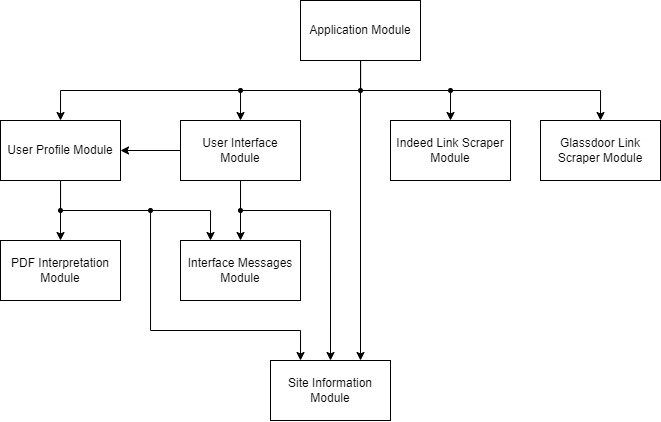
\includegraphics[width=0.7\textwidth]{UsesHierarchy.jpg} 
\caption{Use hierarchy among modules}
\label{FigUH}
\end{figure}

\bibliographystyle {plainnat}
\bibliography {MG}

\end{document}